\documentclass[
%% TIKZ_CLASSOPTION %%
tikz
]{standalone}
\usepackage{amsmath}
\usetikzlibrary{matrix}
%% EXTRA_TIKZ_PREAMBLE_CODE %%
\begin{document}
%% TIKZ_CODE %%
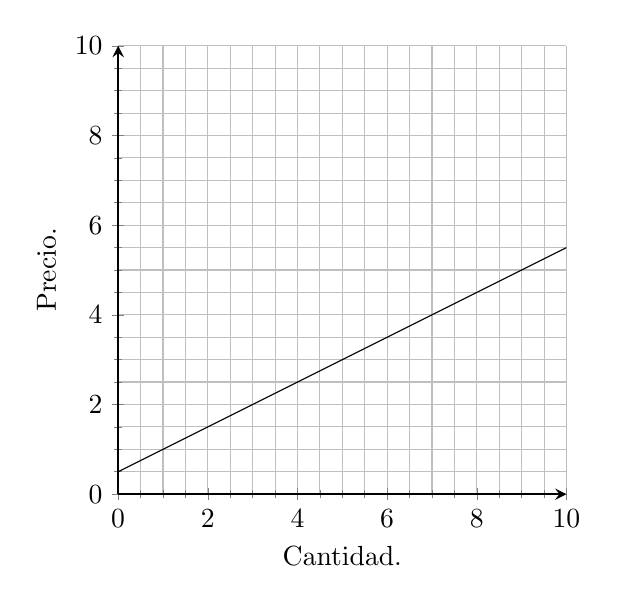
\begin{tikzpicture}
	\begin{axis}[grid=both,
	unit vector ratio*=1 1 1,
	axis x line=bottom,
	axis y line=left,
	axis line style=thick,
	xmax=10,xmin=0,
	ymax=10,ymin=0,
	xtick={0,2,4,6,8,10},
	ytick={0,2,4,6,8,10},
	minor tick num=3,
	xlabel=Cantidad.,
	ylabel=Precio.,
	ylabel near ticks,
	ylabel style={align=center},
	xlabel near ticks,
	]
	
	\addplot[draw, smooth] coordinates {(0,0.5) (10,5.5)};
	\end{axis}
\end{tikzpicture}
\end{document}
